% Created 2018-07-11 Wed 11:38
% Intended LaTeX compiler: pdflatex
\documentclass[11pt]{article}
\usepackage[utf8]{inputenc}
\usepackage[T1]{fontenc}
\usepackage{graphicx}
\usepackage{grffile}
\usepackage{longtable}
\usepackage{wrapfig}
\usepackage{rotating}
\usepackage[normalem]{ulem}
\usepackage{amsmath}
\usepackage{textcomp}
\usepackage{amssymb}
\usepackage{capt-of}
\usepackage{hyperref}
\date{\today}
\title{}
\hypersetup{
 pdfauthor={},
 pdftitle={},
 pdfkeywords={},
 pdfsubject={},
 pdfcreator={Emacs 26.0.91 (Org mode 9.1.13)}, 
 pdflang={English}}
\begin{document}

\tableofcontents

\section{Personalmanagement}
\label{sec:orgf6885d8}
\subsection{Personal \& Wettbewerbsfähigkeit}
\label{sec:orga9c3719}
Das Ausgangsproblem dreht sich um die optimale Ergiebigkeit menschlicher Arbeitsleistung (Gutenberg).

Kategorien/Ebenen personalwirtschaftlichen Handelns:
\begin{itemize}
\item Zielebene = Verfügbarkeit \& Wirksamkeit von Personal
\item Instrumentenebene = Selektion personalwirtschaftlicher Maßnahmen (Instrumente/Ergebnisse) und ihre Wirkungen (intendiert / nicht intendiert)
\item Erfolgsebene = Management der Humanressourcen und Unternehmenserfolg
\end{itemize}

\begin{enumerate}
\item Personalwirtschaftliches Handeln
\label{sec:orga9d796b}
Geht man davon aus, dass ein bestimmter personalwirtschaftlicher Zweck prinzipiell durch verschiedene Handlungen erreicht werden kann, dass außerdem eine bestimmte Handlung prinzipiell verschiedenen personalwirtschaftlichen Zwecken dienen kann und dass schließlich Handlungen auch 'nicht-bezweckte'(nicht-intendierte) Wirkungen hervorrufen können, so werden \emph{Wahlprobleme} sichtbar, die sich mit Hilfe von elementaren \emph{Kategorien} charakterisieren lassen.

Personalwirtschaftl. Probleme entstehen, wenn Unternehmer andere Personen zur Deckung des Arbeitskräftebedarfs in einer Weise in Dienst stellen dass diese bestimmte Dispositionsbefugnisse über ihre Arbeitskraft gegen eine festgelegte Vergütung direkt oder indirekt auf den Unternehmer übertragen.

Prolemkategorien:
\begin{itemize}
\item Herstellung \& Sicherung der Verfügbarkeit \emph{über} Personal (\textbf{Disponibilität})
\begin{itemize}
\item menschliche Arbeitskraft ist ein knappes "Gut"
\item menschliche Arbeitskraft wird in versch Qualität nachgefragt \& angeboten
\item der Bedarf des Betriebes an Personal verändert sich quantitativ und/oder strukturell
\item eine zu einem bestimmten Zeitpunkt gegebene Ausstattung eines Betriebes mit Personal unterliegt im Zeitablauf quantitativen und/oder strukturellen Veränderungen, die nicht durch betriebliche Dispositionen induziert werden
\end{itemize}
\item Herstellung \& Sicherung der Verfügbarkeit \emph{des} Personal (\textbf{Funktionalität})
\begin{itemize}
\item Ansprüche an das Verhalten des Personals sind je nach Situation bzgl ihres konkreten Inhalts und ihres relativen Gewichts unterschiedlich
\item Personal wird idR aufgrund von Selbstdarstellung, Fremdeinschätzung \& Verhaltensstichproben ausgewählt, deren Aussageberich beschränkt und deren Aussagekraft häufig gering sind
\item die Annahme, das sich die Arbeitskräfte mit den Verhaltensansprüchen der Organisation identifizieren, trifft im Regelfall weder für die Verhaltensansprüche noch für alle Angehörigen eines Betriebens in gleicher Weise zu
\item die Erfüllung von Verhaltensansprüchen muss den Mitarbeitern möglich sein
\end{itemize}
\end{itemize}

\item Instrumentenebende personalwirtschaftlichen Handelns
\label{sec:org945b2e8}
\begin{figure}[htbp]
\centering
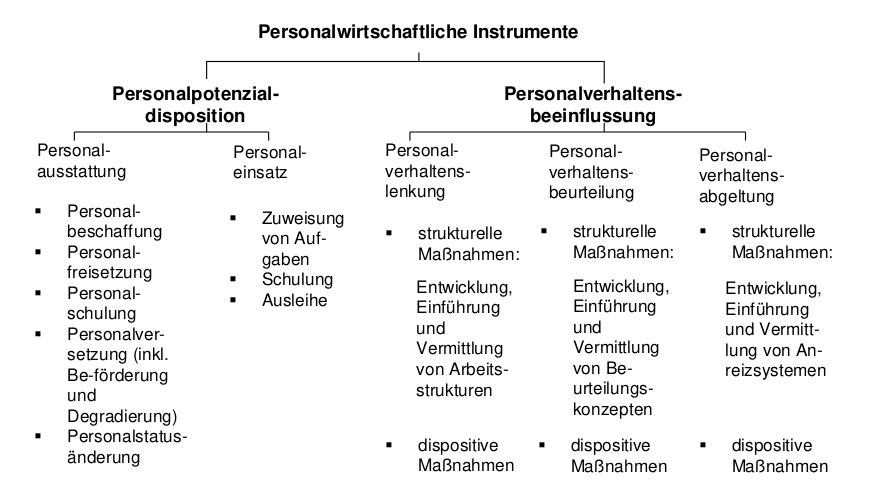
\includegraphics[width=250px]{./pictures/persinstr.png}
\caption{Instrumentenebene personalwirtschaftlichen Handelns}
\end{figure} 

\item Zielebene personalwirtschaftlichen Handelns
\label{sec:org7d28a0b}
\begin{itemize}
\item Individuelle Schutzreche
\begin{itemize}
\item Schutz des Arbeitsverhältnisses (zB Kündigungsschutz)
\item Schutz der Gesundheit (zB Emissionschutz, Arbeitsschutz)
\item besondere Schutzrechte (zB für gefährdete Mitarbeitergruppen)
\end{itemize}
\item Arbeitsrechtliche Mitbestimmung
\begin{itemize}
\item Beteiligung bei sozialen \& personellen Entscheidungen
\item Informations-, Beratungs-, Mitwirkungs- und Mitbestimmungsrechte
\item Interessenvertretung durch Betriebsrat, Jugendvertretung, Wirtschaftsausschuss oä
\end{itemize}
\item Unternehmerische Mitbestimmung
\begin{itemize}
\item Mitwirkungsrechte bei unternehmerischen Entscheidungen
\end{itemize}
\end{itemize}

\item Erfolgsebene personalwirtschaftlichen Handelns
\label{sec:orgd825129}

\item Elementarkategorien personalwirtsch Handelns (Zusammenfassung)
\label{sec:org182f75c}
\begin{figure}[htbp]
\centering
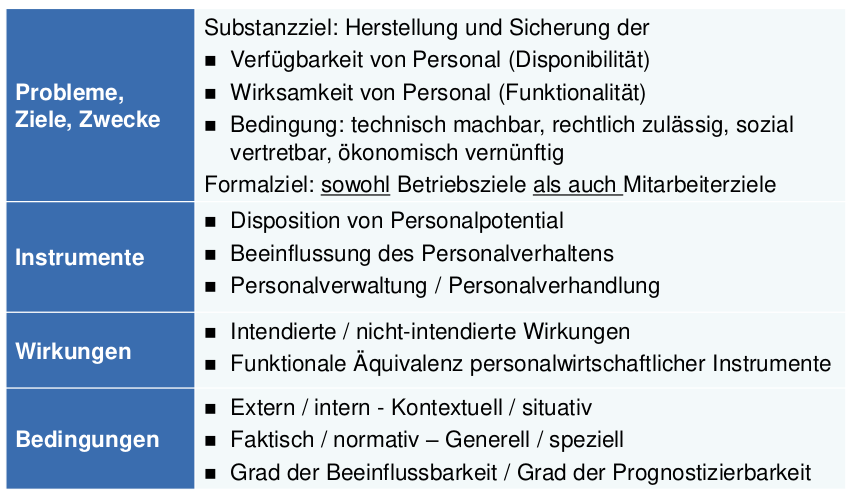
\includegraphics[width=250px]{./pictures/perskateg.png}
\caption{Instrumentenebene personalwirtschaftlichen Handelns}
\end{figure}
\end{enumerate}

\subsection{Disposition des Personalpotentials}
\label{sec:orgab2b521}
\begin{enumerate}
\item Personalrekrutierung und -auswahl
\label{sec:org0df98bb}
Der \emph{Personalbedarf}
\item Personalentwicklung
\label{sec:org13220f9}
\end{enumerate}
\subsection{Beeinflussung des Personalverhaltens}
\label{sec:org41c1f83}
\begin{enumerate}
\item Motivation \& Motivationsprozesse
\label{sec:orgb88151d}
\item Motivation durch Anreizsystme und Arbeitsgestaltung
\label{sec:org62ff121}
\end{enumerate}
\end{document}
